\mychapter{Termo de Autorização do Autor}
\label{Cap:anexo}

A principal diferença entre anexo e apêndice é que os apêndices são textos criados pelo próprio autor para complementar sua argumentação, enquanto os anexos são documentos criados por terceiros e usados pelo autor.

Tanto o apêndice quanto o anexo devem estar presentes no sumário dos trabalhos científicos. Os apêndices devem aparecer depois das referências e os anexos depois dos apêndices.

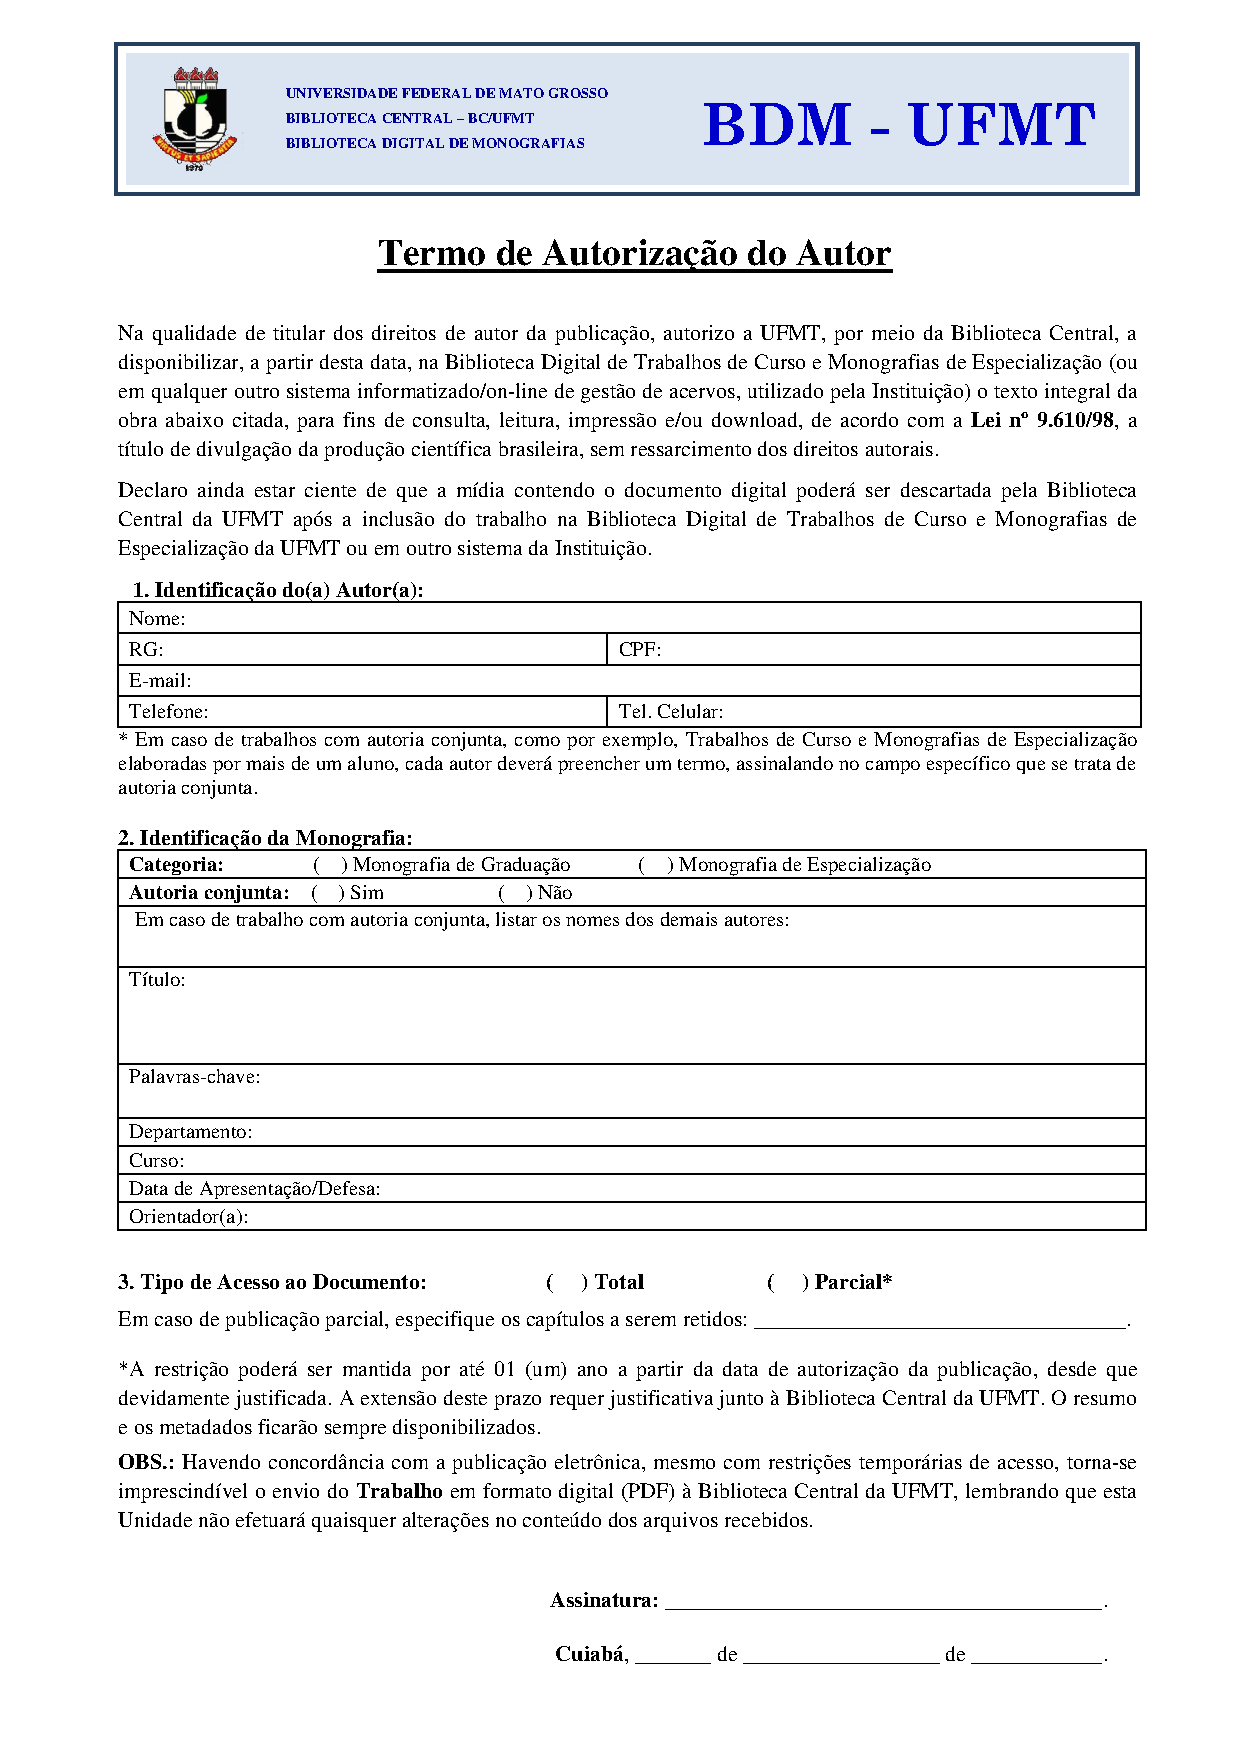
\includepdf[pages=-]{textuais/anexo/termo_de_autorizacao.pdf}

\mychapter{Configuração da Máquina de Desenvolvimento}
\label{Ap:configuracaoMaquina}

Este apêndice apresenta as especificações de hardware e software da máquina utilizada para o desenvolvimento do sistema RADARE, garantindo que o ambiente fosse adequado para o trabalho de desenvolvimento e testes do \textit{software}.

\section{Especificações de Hardware}
\begin{itemize}
    \item \textbf{Processador}: Intel Core i7-10750H (2.6 GHz até 5.0 GHz, 6 núcleos)
    \item \textbf{Memória RAM}: 16 GB DDR4
    \item \textbf{Armazenamento}: 512 GB SSD NVMe
    \item \textbf{Placa Gráfica}: NVIDIA GeForce GTX 1650 Ti (4 GB GDDR6)
    \item \textbf{Monitor}: Resolução Full HD (1920x1080) em uma tela de 15,6 polegadas
\end{itemize}

\section{Especificações de Software}
\begin{itemize}
    \item \textbf{Sistema Operacional}: Windows 11 Pro (64-bit)
    \item \textbf{Editor de Código}: Visual Studio Code (com extensões para TypeScript, Python e controle de versão Git)
    \item \textbf{Versionamento de Código}: Git e GitHub para controle de versão e colaboração
    \item \textbf{Ambiente de Execução de Python}: Python 3.9 com bibliotecas específicas para o desenvolvimento \textit{back-end}
    \item \textbf{Navegadores para Testes}: Microsoft Edge, Google Chrome e Mozilla Firefox (versões mais recentes)
\end{itemize}

\section{Extensões Utilizadas no Visual Studio Code}
\begin{itemize}
    \item \textbf{TypeScript}: Extensão para suporte e autocompletar do TypeScript
    \item \textbf{Python}: Suporte ao desenvolvimento com Python, incluindo linting e debugging
    \item \textbf{Prettier - Code Formatter}: Ferramenta de formatação automática para o código
    \item \textbf{ESLint}: Análise de código estática para manter a qualidade do código
    \item \textbf{GitLens}: Ferramenta para integração avançada com Git
\end{itemize}

Essas configurações e ferramentas foram essenciais para assegurar um fluxo de trabalho eficiente, com suporte adequado para o desenvolvimento e teste do \textit{software} RADARE.


\mychapter{Código Completo da Rota POST /reconcile}
\label{Anexo:CodigoRouteReconcile}

\begin{minted}[fontsize=\small, linenos, frame=single, caption={Implementação da Rota POST /reconcile}]{python}
from flask import Flask, request, jsonify
from your_database_module import store_reconciled_data
from your_reconciliation_module import perform_lagrange_reconciliation

app = Flask(__name__)

@app.route('/reconcile', methods=['POST'])
def reconcile_data():
    try:
        # Recebe os dados do front-end em formato JSON
        data = request.get_json()

        # Processa os dados utilizando o método dos multiplicadores de Lagrange
        reconciled_data = perform_lagrange_reconciliation(data)

        # Armazena os dados reconciliados no banco de dados
        store_reconciled_data(reconciled_data)

        # Retorna uma resposta de sucesso ao front-end
        return jsonify({"status": "success", "reconciled_data": reconciled_data}), 200

    except Exception as e:
        # Em caso de erro, retorna uma mensagem de erro
        return jsonify({"status": "error", "message": str(e)}), 500

if __name__ == '__main__':
    app.run(debug=True)
\end{minted}

Este código demonstra como os dados são recebidos e processados pela rota \texttt{POST /reconcile}, aplicando o método de reconciliação e armazenando os resultados no banco de dados para uso posterior.

\mychapter{Código Completo da Rota GET /results}
\label{Anexo:CodigoRouteResults}

\begin{minted}[frame=lines, fontsize=\small, linenos]{python}
from flask import Flask, jsonify
from your_database_module import retrieve_reconciled_data

app = Flask(__name__)

@app.route('/results', methods=['GET'])
def get_results():
    try:
        # Recupera os dados reconciliados do banco de dados
        reconciled_data = retrieve_reconciled_data()

        # Retorna os dados reconciliados para o front-end
        return jsonify({"status": "success", "reconciled_data": reconciled_data}), 200

    except Exception as e:
        # Em caso de erro, retorna uma mensagem de erro
        return jsonify({"status": "error", "message": str(e)}), 500

if __name__ == '__main__':
    app.run(debug=True)
\end{minted}

Este código ilustra como a rota \texttt{GET /results} foi configurada para recuperar os dados reconciliados do banco de dados e enviar essas informações para o \textit{front-end}. O processo inclui a captura de dados previamente ajustados pelo método de reconciliação, permitindo que sejam exibidos na interface de forma organizada para análise.

\mychapter{Código Completo da Rota POST /upload}
\label{Anexo:CodigoRouteUpload}

\begin{minted}[frame=lines, fontsize=\small, linenos]{python}
from flask import Flask, request, jsonify
import csv
from your_database_module import store_csv_data

app = Flask(__name__)

@app.route('/upload', methods=['POST'])
def upload_file():
    try:
        # Verifica se o arquivo foi enviado na requisição
        if 'file' not in request.files:
            return jsonify({"status": "error", "message": "No file provided"}), 400

        file = request.files['file']
        
        # Lê o conteúdo do arquivo CSV
        csv_data = []
        with open(file.stream, 'r') as csvfile:
            csv_reader = csv.reader(csvfile)
            for row in csv_reader:
                csv_data.append(row)

        # Armazena os dados CSV no banco de dados
        store_csv_data(csv_data)

        # Retorna uma resposta de sucesso ao front-end
        return jsonify({"status": "success", "message": "File uploaded successfully"}), 200

    except Exception as e:
        # Em caso de erro, retorna uma mensagem de erro
        return jsonify({"status": "error", "message": str(e)}), 500

if __name__ == '__main__':
    app.run(debug=True)
\end{minted}

Este código descreve a implementação da rota \texttt{POST /upload}, responsável pelo processamento de arquivos CSV enviados pelo \textit{front-end}. Os dados do arquivo são lidos, processados e armazenados no banco de dados, permitindo que sejam utilizados nas etapas subsequentes de reconciliação e análise.
